\documentclass[a5paper]{article}

\usepackage{amsmath, amssymb}
\usepackage{multicol}
\setlength{\columnsep}{1cm}
\usepackage[margin=0.75in]{geometry}
\usepackage{graphicx}
\graphicspath{ {../../../Images/COIT12209/} }
\usepackage[breaklinks, hidelinks]{hyperref}
\usepackage{siunitx}
\usepackage{tikz}
\usetikzlibrary{positioning, arrows.meta}
\usepackage{pgfplots}
\pgfplotsset{compat=newest}
\usepgfplotslibrary{external}
\usepackage{stix}
\usepackage{ragged2e}
\usepackage{enumitem}
\usepackage{polynom}

\newcommand{\sech}{\mathrm{sech}}
\newcommand{\csch}{\mathrm{csch}}
\setcounter{secnumdepth}{4}
\renewcommand\paragraph{\@startsection{paragraph}{4}{\z@}%
% display heading, like subsubsection
                                     {-3.25ex\@plus -1ex \@minus -.2ex}%
                                     {1.5ex \@plus .2ex}%
                                     {\normalfont\normalsize\bfseries}}
\sisetup{
	round-mode = places,
	round-precision = 2,
}

\date{18\textsuperscript{th} of June 2026}

\begin{document}
	\begin{titlepage}
		\centering
		{\Huge \textsc{COIT12209}\par}
		\vspace{1cm}
		{\Large \textsc{Lecture Notes}\par}
		\vspace{2.5cm}
		\vfill
		Authored by\par
		Lachlan J. W. Wyer
		\vfill
		\makeatletter
		{\large Document Start Date: \@date \par}
		\makeatother
		{\large Latest Update: \today\par}
	\end{titlepage}
	\tableofcontents
	\pagebreak

	\section{What is Data Science?}
	\subsection{Data Science:}
	The collection, preperation, analysis, visualization, management and presentation of large collections of data. Data science specifically is the exploration of data via the scientific method. It  is crucial we understnad data science as we are in an age where everything is going digital. For example, targeted advertising and sponsored results.
	\subsection{History of Data Science:}
	FAANGY (Facebook, Apple, Amazon, Netflix, Google and Yahoo!) realised they have copious amount of data laying around. If they applied machine lear\-ning techniques to the data, significant business benefits occur. These can include better product recommendations, fraudulant activity monitoring, and click through rates.
	\subsection{Data Science Sub-Fields:}
	\begin{itemize}
		\item Mathematics and Statistics
		\item Machine Learning
		\item Software Engineering
		\item Domain Knowledge
	\end{itemize}
	\subsection{What is Data?:}
	Data usually refers to raw/unprocessed facts. Once anything is done to these facts, in way normies can understand, these facts are considered information.
	\subsubsection{Data Types}
	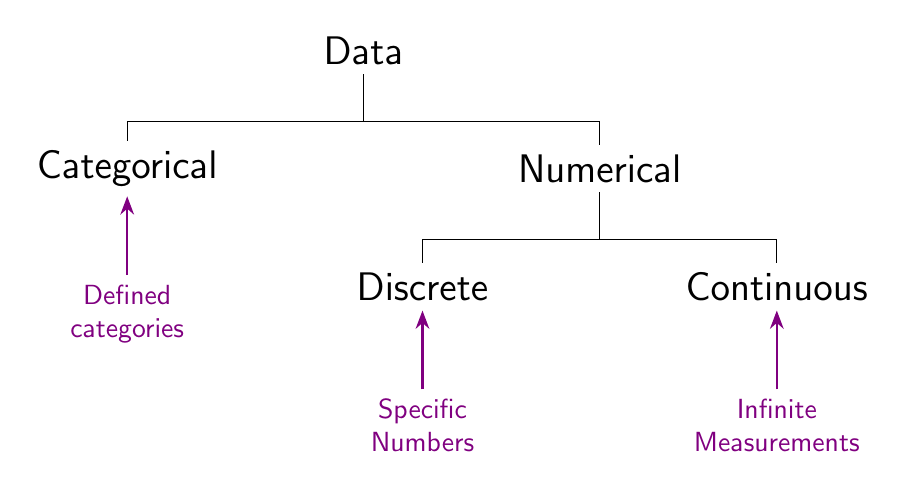
\begin{tikzpicture}[
	    % Style for the orthogonal branching lines
	    edge from parent path={(\tikzparentnode.south) -- +(0,-0.6cm) -| (\tikzchildnode.north)},
	    level 1/.style={sibling distance=6cm, level distance=1.5cm},
	    level 2/.style={sibling distance=4.5cm, level distance=1.5cm},
	    % Styles for text nodes and annotation lines
	    main node/.style={font=\Large\sffamily, text=black},
	    annotation/.style={font=\normalsize\sffamily, text=violet, align=center},
	    arrow/.style={->, >=Stealth, thick, violet}
	]

	% Main tree structure
	\node[main node] {Data}
	    child { node[main node] (cat) {Categorical} }
	    child { node[main node] (num) {Numerical}
		child { node[main node] (disc) {Discrete} }
		child { node[main node] (cont) {Continuous} }
	    };
	% Purple annotations with upward arrows
	\node[annotation, below=1cm of cat] (cat_ann) {Defined\\categories};
	\draw[arrow] (cat_ann) -- (cat);

	\node[annotation, below=1cm of disc] (disc_ann) {Specific\\Numbers};
	\draw[arrow] (disc_ann) -- (disc);

	\node[annotation, below=1cm of cont] (cont_ann) {Infinite\\Measurements};
	\draw[arrow] (cont_ann) -- (cont);
	\end{tikzpicture}
	\subsection{Big Data:}
	Comprised of 3 main characteristics:
	\begin{enumerate}
		\item Volume
		\item Velocity
		\item Variety
	\end{enumerate}
	Structured Big Data is the common. The formats this comes in is SQL, or CSVs. The positives of these formats is that they can be easily searched. However, must follow strict schema, offering limited flexibility.\\
	Semi-structured have a litt bit of organization like tags or keys, but does not follow strict schema rules. This giver more flexibility too the data but makes it harder to query. Formats can include XML, YAML, and JSON.\\
	Unstructured data follows no consistent formatting. These include text files, PDFs and A/V files. They are rich in formation but hard to store and query efficiently.\\
	Big Data plays a crucial role in industry as it allows data driven descion making.

	\section{Identifying Data}
	\subsection{Data Mining Task:}
	Data mining tasks are specific operations or processes to find extra patterns or insights from the data. By breaking down big data into smaller chunks an easier insight can be found. This allows humans to only do the part where creativity can be found, I.E engaging with stakeholders.
	\subsection{Business Problems:}
	Business analystics and problem solving require data scientists to find "cor\-relations" between variables, their meanings and relationships to other variables. In additon it allows informed descion making based on a data driven approach.
	\subsection{Data Mining Task:}
	Data mining taks are designed to extract insights or knowlegde from a data set. This is split into 2 categories:
	\begin{enumerate}
		\item Predictive tasks: Use historic data to predict future values
		\item Descriptive tasks: Discovering patterns without prior labels
	\end{enumerate}
	\subsubsection{Predictive Tasks}
	\begin{itemize}
		\item Classification and class probability: Predicting a category label for each instance.
		\item Regression: Predict a continuous numeric value.
		\item Similarity matching: Predict which past records are most alike a new input.
		\item Link prediction: Predicting future or missing connections in a network.
		\item Casual modeling: Estimation of the effect of an invention.
	\end{itemize}
	\subsubsection{Descriptive Tasks}
	\begin{itemize}
		\item Clustering: Discovering groupings or clustering within data sets.
		\item Co-occurence grouping: Items found frequently together.
		\item Profiling (Behaviour description): Describes typical behaviour within a group.
		\item Data reduction: Simplify or compress data while preserving key information.
	\end{itemize}
	\subsection{Classification:}
	Predicting discrete class labels from the class probability. That being the likelihood that an instance belongs to a particular class.
	\subsection{Data Collection:}
	\begin{enumerate}
		\item Manual Collection
			\begin{itemize}
				\item Observing and recording
				\item Interviews
				\item Questionares
				\item Pros:
					\begin{itemize}
						\item Fine-tuned
						\item Accurate
					\end{itemize}
				\item Cons:
					\begin{itemize}
						\item Scale
						\item Cost
						\item Reachablility
					\end{itemize}
			\end{itemize}
		\item Automatic Approach
			\begin{itemize}
				\item Transaction history or logs
				\item Sensors suchas, GPS, IoT or Lab equipment
				\item Web crawler
				\item Social media
				\item Pros:
					\begin{itemize}
						\item Mass collection
						\item Easy
						\item Cheap on a large scale
					\end{itemize}
				\item Cons:
					\begin{itemize}
						\item Mass collection comes with increased mess
					\end{itemize}
			\end{itemize}
	\end{enumerate}
	\subsection{Sampling:}
	Data sampling is a statistical analysis technique used to select, manipulate and analyse a subset of representative data. This is done to reduce compute time, resource allocation, and time limits. Sampling types include:
	\begin{itemize}
		\item Simple random sampling
		\item Stratified sampling
		\item Cluster sampling
		\item Systematic sampling
		\item Multi-stage sampling
	\end{itemize}
	\subsection{Data Mining Process:}
	Industry standard is CRIP-DM. This stands for Cross Industry Standard Process for Data Mining.

	\section{Ethics and Law}
	\subsection{Ethics, Morality and Law:}
	Ethics is purely a branch of philosophy that consist of a set of values to define the rightness and wrongness of an action. Morality is th ethics and belief held by a group, and usually constituated from cultural and relgious principles. Law is defined by a set of rules determined by a governing body. Usually informed through legal instituation and carries consequence to those who break it.
	\subsection{Organizational Evil:}
	OE involves systemic or institutional wrong doing that harms consumers. Basically designed to maximise a companies profits. OE can take various forms:
	\begin{itemize}
		\item Unethical practices
		\item Abusive behaviour
		\item Corruption
		\item Disegard to human-rights.
	\end{itemize}
	\subsection{Digital Era Bias:}
	Bias is shown through favouritism toward opinions, action or descions.
	\begin{enumerate}
		\item Algorithmic Bias: AI powered systems ignore bias training data to favour particular outcomes.
		\item Sampling Bias: Showed dataset containing societal inequalities. Usually happens because of wrong sampling processes.
		\item Confirmation Bias: Recommendations enforcing existing beliefs.
		\item Representation Bias: Occurs when certain groups or characteristics are over represented.
		\item Accessibility Bias: Design choices affecting those with a disability.
		\item Language Bias: LLMs may exhibt a bias towards a particular language.
	\end{enumerate}
	\subsection{Gen AI Ethics:}
	Gen AI should address concerns related to its generated content.
	\subsection{Ethical Dilemma:}
	This occurs when tow or more ethical principles conflict. A solution can be difficult to find.
	\subsection{Ethical Data Science:}
	EDS refers to a set of moral principles and guidelines outlining data use. Its about making companies think about utilizing data fairly. Australia subscribes to the follow 10 rules for data research:
	\begin{enumerate}
		\item Acknowledge that data are people and can do harm.
		\item Recognize that privacy is more than a binary value.
		\item Guard against the reidentification of your data.
		\item Practice ethical data sharing.
		\item Consider the strengths and limitations of your data; big data does not automatically mean better.
		\item Debate the tough, ethical choices.
		\item Develop a Code of Conduct for your organization, research community, or industry.
		\item Design your data and systems for auditability.
		\item Engage with the broader consequences of data and analysis practices.
		\item Know when to break these rules.
	\end{enumerate}

	\section{Data Presentation}
	\subsection{Data and Computers:}
	Computers deal with many different types of data when processing commands and presenting answers. These can be text, audio, video or pictures.
	\subsection{Analog and Digital:}
	Information is presented in 2 main ways:
	\begin{enumerate}
		\item Analog: A continuous representation that changes smoothly over time.
		\item Digital: Discrete values, that are broken up using binary code.
	\end{enumerate}
	\subsection{Representing Data:}
	\subsubsection{Text}
	The most common is the ASCII set. Since its introduction in 1968 it has become the default way of doing text with 1Byte per character. 
	\subsubsection{Audio}
	Soundwaves are an analog signal. Computers need to convert the analog signal to digital for storage and back again for use. It does this through taking small discrete samples at regular intervals.
	\subsubsection{Video}
	A video file consists of multiple sub files. Suchas, photos, audio, and subtitles.
	\subsection{Effictive Presentation:}
	Raw and processed is not interesting or easy to understand for normies. Making this data easy to digest and understand is critical. Effective data presentation follows the following principles; clear, concise, attractive and attentionable.

	\section{Data Analytics}
	\subsection{What is it?:}
	Data analytics is simply the study of data to answer business questions. Not just about more data but a look at the same data. It can be simply put in 5 key principles:
	\begin{enumerate}
		\item Define the analytical problem clearly
		\item Collaborate with quantative experts
		\item Recognize data types and their impact
		\item Apply the right type of analytics
		\item Leverage analytics internally and externally
	\end{enumerate}
	\subsection{Exploratory Data Analytics:}
	This is about getting an overall sense of the dataset. Some of the ways this is done is through visualization and 5-number summaries. This is especially useful in early stages of data mining, finding outliers, missing values and testing assumptions. EDA measures 2 main things:
	\begin{enumerate}
		\item Central tendency: Report a single dat point that describes the most typical response
		\item Variability: The typical difference between data points
	\end{enumerate}
	\subsection{Descriptive Modelling:}
	It looks towards the "what happened" to cause the data trends.
	\subsubsection{Association Rules}
	\begin{itemize}
		\item If/then statements to uncover relationships between data points
		\item Data sources
		\item Results: Dependency rules which predict occurrence of some items\\based on others
	\end{itemize}
	\subsubsection{Clustering Analysis}
	\begin{itemize}
		\item Group data points together that
			\begin{itemize}
				\item Are more similar to one another
				\item In seperate clusters not alike each other
			\end{itemize}
		\item Similarity Measurements
			\begin{itemize}
				\item Euclidean distance
				\item Problem-specific measurements
			\end{itemize}
	\end{itemize}
	\subsection{Diagnostic Analysis:}
	The process behind understanding the causes and reasons behind why a certain event happens. Diagnostic and descriptive analysis work together to find the answer.
	\subsection{Predictive:}
	Based on previous history and performance, how is the likelihood going to occur.
	\subsection{Perscriptive:}
	Looks forwards for a best course of action based on data analysis.
	\subsection{Approach to Enterprise Analytics:}
	\begin{itemize}
		\item Define business objectives
		\item Data strategy and governance
		\item Infrastructure and tools
		\item Data integration and centralization
		\item Advanced analytics
		\item Data visualization and reporting
		\item Cross-functional collaboration
		\item Continuous learning
		\item Feedback and iteration
	\end{itemize}

	\section{Data Discovery and Mining}
	\subsection{Data Driven Descions:}
	The process a business makes when taking critical descions, based on reliable data, insights and facts. A descion-making approach that collect analyses and interprets data around KPIs.
	\subsection{Data Discovery:}
	The real starting point, starts with a question before data is associated.
	\subsection{Data Selection:}
	\begin{itemize}
		\item Identify relevant data sources for the problem
		\item Choose attributes that are meaningful
		\item Ensure data is representative of domain
	\end{itemize}
	\subsection{Data Cleaning:}
	\begin{itemize}
		\item Handle missing values
		\item Detect inconsistencies and errors
		\item Remove duplicates
		\item Address noise, filler and outliers
		\item Standardise formats
	\end{itemize}
	\subsection{Data Transformation:}
	\begin{itemize}
		\item Feature creation: Generate new attributes to capture useful patterns
		\item Data reduction: Simplify data sets using dimensionality reduction
		\item Data normalisation and scaling: Adjust values to a common scale for improved comparability
		\item Data encoding: Convert categorical into numerical values
		\item Aggregation/Discretion: Combine on group values
	\end{itemize}
	\subsection{Data Mining:}
	A core step of KDD: apply computational techniques to extract patterns, trends or models to data. These methods include:
	\begin{itemize}
		\item Classification: Predict categories
		\item Regression: Predict continuous values
		\item Clustering: Group similar records
		\item Association Rules: Find co-occurance patterns
		\item Anomaly Detection:  Identify unusual cases
	\end{itemize}
	\subsection{Interpretation and Evaluation:}
	\begin{itemize}
		\item Interpret results
		\item Evaluate usefulness
		\item Validate models
		\item Compare alternatives
		\item Communicate findings
	\end{itemize}
	\subsection{Data Mining Approach:}
	A verification driven process:
	\begin{itemize}
		\item Validates a hypothesis
		\item Querying and reporting
		\item Multi-dimensional analysis
		\item Statistical Analysis
	\end{itemize}
	It focuses on data-driven discoveries:
	\begin{itemize}
		\item EDA
		\item Predictive Modelling
		\item DB segmentation
		\item Link analysis
		\item Deviation detection
	\end{itemize}
	\begin{center}
		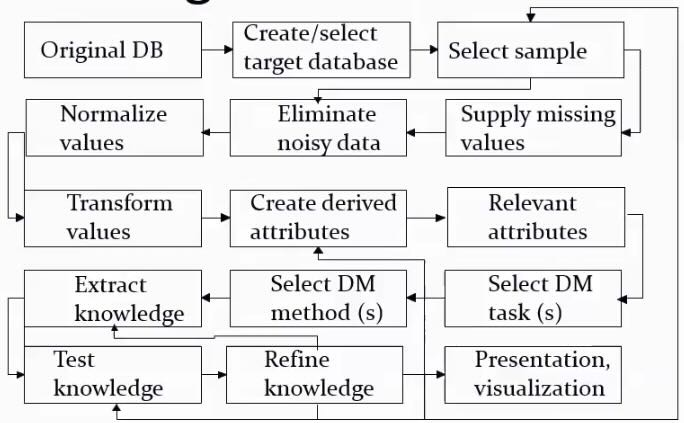
\includegraphics[scale=0.5]{data-mining-approach.png}
	\end{center}
	\subsection{Why Data Mining?:}
	Human analysis breaks down with increased volumn and dimensionality.\\Works to be done by non-staticians.
	\subsection{Data Mining Techniques:}
	\begin{itemize}
		\item Association Rules: Detects attributes frequenty found together
		\item Sequence Mining: Discovers event sequences that occur together
		\item Similarity Search: Given a DB of objects and a query. Find all occurences within a user-defined range
		\item Deviation Detection: Find records that are most different from the rest
		\item Classification and Regression: Assign a new data record to one of several predefined categories or classes
		\item Clustering: Partition the dataset into subgroups that have common sets of properties
	\end{itemize}
	\subsection{Data Mining Models:}
	\begin{itemize}
		\item Descion Trees
		\item Random Forrest
		\item Nueral Network
		\item K-means Clustering
		\item K-nearest neighbours
		\item Apriori and FP-Growth
		\item Sequence Mining Techniques
	\end{itemize}
	\subsection{Data Mining Types:}
	General descriptive knowledge:
	\begin{itemize}
		\item Summarization
		\item Symbolic descriptions of subsets
	\end{itemize}
	Discriminative knowledge:
	\begin{itemize}
		\item Distinguish K-classes
		\item Accurate classification
		\item Seperate space
	\end{itemize}
	\subsection{Components of Data Mining Methods:}
	\begin{itemize}
		\item Representation: Language for patterns or models
		\item Evaluation: Scoring methods for deciding what is a good of model to data
		\item Search: Method for enumerating patterns or models
	\end{itemize}

	\section{Exploratory Data Analytics}
	\subsection{Analysis:}
	The process of looking at data and showing it in tables, charts and simple descriptions. This is so that it become useful information. For example, taking raw exams scores and presenting them in a table.
	\subsection{Interpretation:}
	This is understanding what that useful information actually means. Usually done by making connections, comparing results and thinking about reasonable outcomes. Suchas, noticing students who study more achieve better grades and discussing why this might be the case.
	\subsection{How to Interpret Data?:}
	\begin{itemize}
		\item Target: Does result meet a set goal?
		\item Relevance: Why is this finding relevant?
		\item Reason: What might explain this result?
		\item Comparison: How does this result compare with other known good results?
		\item Triangulation: Are there any other datasets that could be checked to confirm this result?
		\item Next Steps: Is deeper analysis required to understand the data?
	\end{itemize}
	\subsection{Trend Analysis:}
	A basic technique used to patterns, trends and outliers in time series data. Insights flagged will be then placed under deeper investigation.
	\subsection{Box Plots:}
	They quickly visualize variations in base data. In addition to quickly identifying outliers. Graphically showing groups of numerical data through their quartiles.
	\subsection{Spatial Analysis:}
	Uses location based data to analyse activities and conditions. For example: Map data
	\begin{itemize}
		\item Roads
		\item Building
		\item Environment
		\item Weather
	\end{itemize}
	\subsection{Pairs Plot:}
	Helps spot potential correlations by comparing variables pair by pair. Uses non-leading diagonal (wher some variables meet) as a historgram or KDE plot. All others are scatter plots with trend lines.
	\subsection{Time Series:}
	Time series is a series of data points in which each data point is associated with a timestamp.
	\subsubsection{Trends}
	\begin{itemize}
		\item Long-term movement of data
		\item Changes of direction
	\end{itemize}
	\subsubsection{Seasonal}
	\begin{itemize}
		\item Regular repeating patterns tied to a calender
		\item Frequency is fixed and predictable
	\end{itemize}
	\subsubsection{Cyclic}
	\begin{itemize}
		\item Longer term rises and falls that are not fixed length
		\item Often linked to business and economic conditions
	\end{itemize}

	\section{Analytics Algorithms}
	An analytical model is statistical model that is designed to perofmr a specific task, or predict the probability of an event. Type include:
	\begin{itemize}
		\item Classification Model
		\item K-means clustering Model
		\item Forecast Model
		\item Nueral Networks
		\item Decision Trees
		\item Logistic Regression
		\item Time-series Regression
	\end{itemize}
	\subsection{Clustering Analysis:}
	CA is the process of grouping a set of objects go that;
	\begin{itemize}
		\item Objects wihin the same group are more similar to each other
		\item Objects in different groups are less similar
	\end{itemize}
	The purpose of CA is the uncover the natural grouping within the data.
	\begin{center}
		\includegraphics[scale=0.5]{ca-example.png}
	\end{center}
	\subsection{K-Means Clustering:}
	One the simplest clustering algorithms.
	\begin{enumerate}
		\item Selects k-number of objects from the dataset, each representing intial cluster centers.
		\item Each object is assigned to the cluster to which is most similar. This is based on distance between object and cluster center.
		\item The means of clusters are computed as new cluster centers.
		\item Function continues until criterion function converges.
	\end{enumerate}
	\subsection{Regression Analysis:}
	Used to predict a continuous value such as the volume of rain. Regression is to build a function of independent variables (predictors) to predict a dependent variable (response).
	\begin{center}
		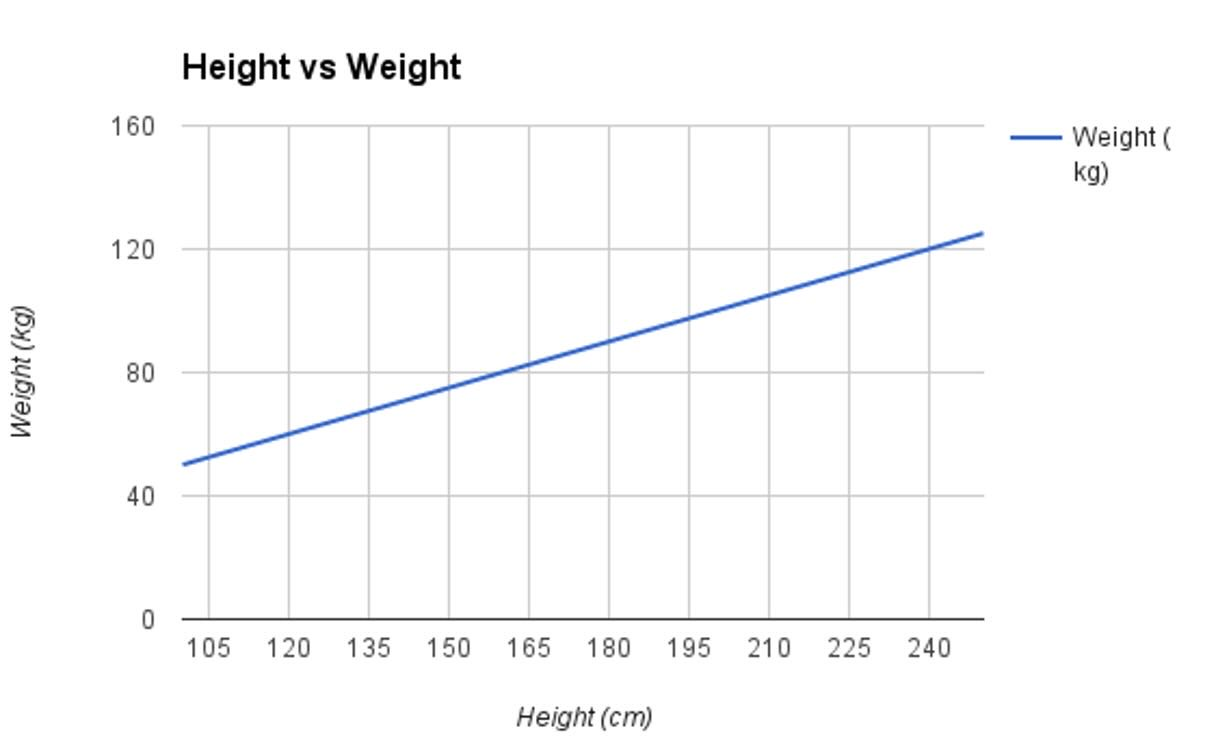
\includegraphics[scale=0.25]{regression-example.png}
	\end{center}
	\subsection{Classifier Analysis:}
	Descision classifier uses a descion tree as a predictive model that maps observations about an item to conclusions about the item's target value.
	\begin{center}
		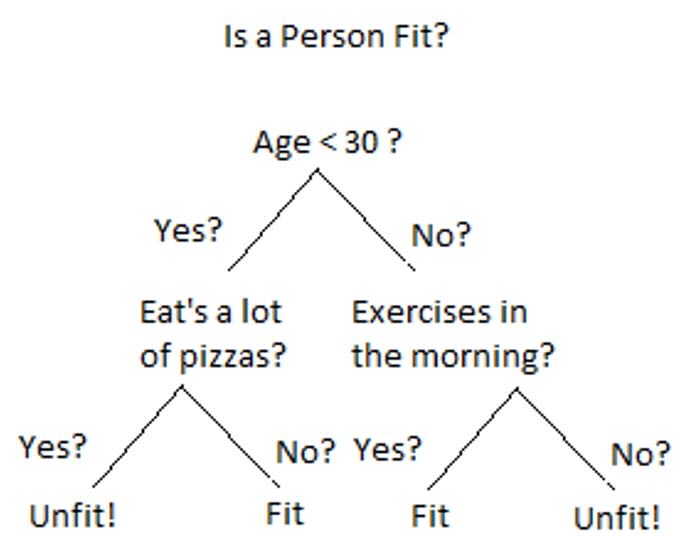
\includegraphics[scale=0.35]{classifier-example.png}
	\end{center}
	\subsection{Association Analysis:}
	A popular algorithm for discovering a quatifying relationships between variables in large DBs. It shows events or activities that tend to happen together. E.g. the market basket analysis.
	\subsection{Graph Analysis:}
	GA uses mathematical structures to model pairwise relations between object. A "graph" in this context is made up of "vertices" or "nodes" and line called edges to connect them.
	\begin{center}
		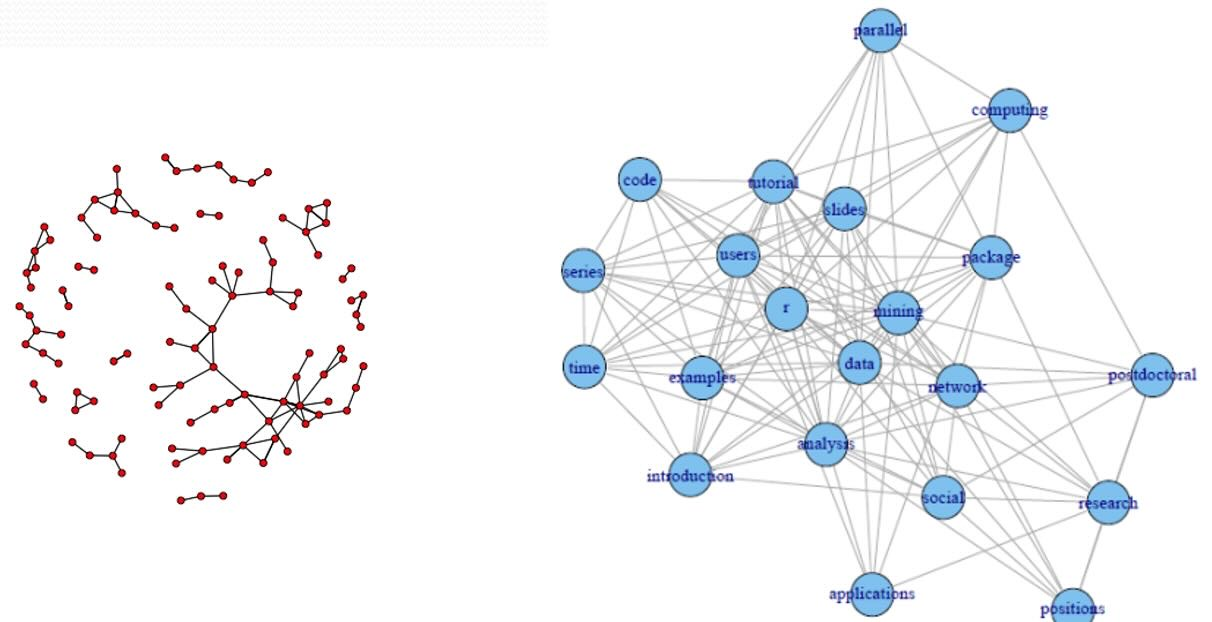
\includegraphics[scale=0.25]{ga-example.png}
	\end{center}
	\subsection{Cohorts Analysis:}
	CohA is the study how cohorts that share common characteristics.
	\begin{center}
		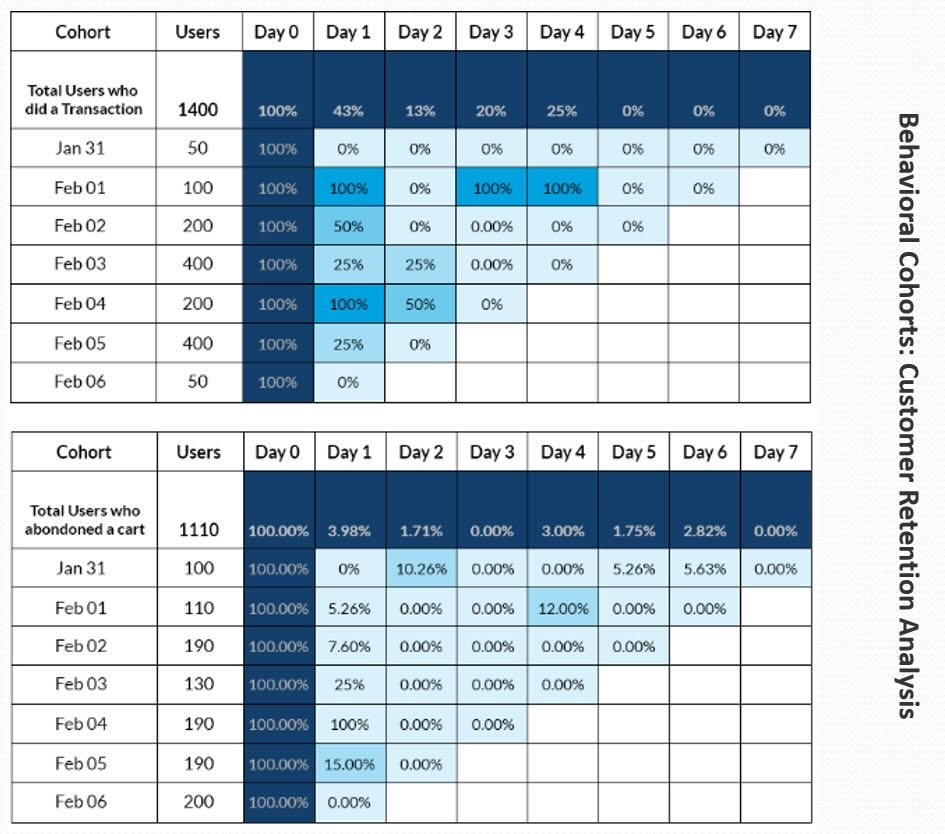
\includegraphics[scale=0.35]{cohort-example.png}
	\end{center}
	\subsection{Traverse Pattern Analysis:}
	TPA is an example of combining multiple analytic algorithms to betten understand patterns.
	\begin{center}
		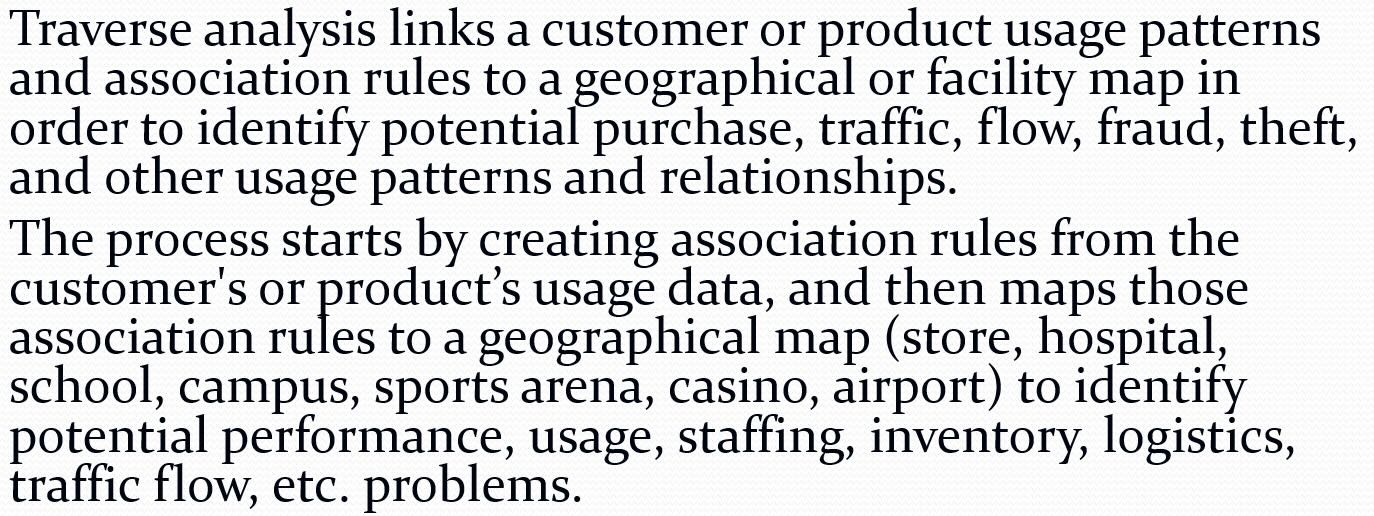
\includegraphics[scale=0.25]{tpa-example.png}
	\end{center}

	\section{Data Integrations}
	No particularily related to EDA and ML but still a crucial part of the learning process.
	\subsection{Objectives:}
	\begin{itemize}
		\item Why do we integrate data?: Understand business and technical drivers for combining multiple data sources.
		\item Challenges to Integration: Issues suchas quality, heterogenity and governences.
		\item ETL Process: Break down extract, transform and load phases in their role of data preperation.
		\item Support Concepts: Know what mapping, staging and meta-data in practice.
		\item Different Approaches: Compare warehousing, federation and virtualization.
	\end{itemize}
	\subsection{What is it?:}
	The process of combining data from different sources to provide a unified and consistent view. The end goal of this is to make data usuable for analytics operations and descion-making.
	\subsection{Why does it matter?:}
	\begin{itemize}
		\item Break down silos: Ensures data is not trapped in seperate systems.
		\item Consistency and quality: Improves trust worthiness of analytics.
		\item Supports descion-making: Executives and analysts see the "big picture".
		\item Operational value: Customer 360 views, supply chain monitoring.
		\item Cross-domain insights - For example, linking health records with genomic data to improve treatment.
	\end{itemize}
	\subsection{Challenges in Data Integration?:}
	Development Issues - Inconsistent field names, missing or duplicated records, and schema mismatches.\\
	Technical Issues - Combining structured and unstructured data, scaling for big data,\\balancing preloaded and real-time.\\
	Organgisational Issues - Data ownership, access and permissions and lock of goverance.
	\subsection{Tech in Data Integration:}
	\subsubsection{Traditional ETL Tools}
	\begin{itemize}
		\item Mature and enterprise grade
		\item Provide drag-and-drop design, scheduling and monitoring
		\item Often used in on-prem warehouses
	\end{itemize}
	\subsubsection{Cloud Integration}
	\begin{itemize}
		\item Severless ETL and ELT services
		\item Integrate with cloud storage and cloud warehouses
		\item Offers scalability and pay-as-you-go functionality
	\end{itemize}
	\subsection{ETL:}
	Extract, transform, and load is the primary method used to integrate data from multiple sources to one central one. The Bridge function: connect raw, scattered data to usable, trusted datasets.
	\subsubsection{Supporting ETL}
	Data Mapping:
	\begin{itemize}
		\item Defines how source fields map to target schema
		\item Ensures consistency when merging heterogeneous data
	\end{itemize}
	Data Staging:
	\begin{itemize}
		\item Provides a temporary area to collect, cleanse and compare data before loading
		\item Helps detect changes and pre-aggregate values
	\end{itemize}
	\subsubsection{Data Extraction}
	Logic method - What data is extracted?
	\begin{itemize}
		\item Full extraction
			\begin{itemize}
				\item All records are pulled each time
				\item Costly for large datasets
			\end{itemize}
		\item Incremental Extraction
			\begin{itemize}
				\item Pull new or changed records
				\item Needs change tracking features
			\end{itemize}
	\end{itemize}
	Physical method - How it is done?
	\begin{itemize}
		\item Online (Real-time)
			\begin{itemize}
				\item Direct full from live systems
				\item APIs
				\item RTMP streams
				\item Adds system load
			\end{itemize}
		\item Offline (Batch)
			\begin{itemize}
				\item Export files or snapshots at intervals
				\item Not in real-time
			\end{itemize}
	\end{itemize}
	\subsubsection{Data Trasnformation}
	Most complex step, consisting of the following key tasks:
	\begin{itemize}
		\item Standardisation
		\item Type conversions
		\item De-duplication
		\item Date scrubbing
		\item Enrichment
	\end{itemize}
	\subsubsection{Data Loading}
	Moving transformed data into a target repo. Load types:
	\begin{itemize}
		\item Replace or overwrite
			\begin{itemize}
				\item Old dates discarded and replaced with the newest
				\item Simple
				\item Loses history
			\end{itemize}
		\item Append (Insert)
			\begin{itemize}
				\item New recoreds added to existing dataset
				\item Useful for logs or transactional data
			\end{itemize}
		\item Maintain historical versions
			\begin{itemize}
				\item Store old and new data
				\item Slowly changing dimensions
				\item Supports trend analysis and auditing
			\end{itemize}
	\end{itemize}
	\subsection{Need Data Integration:}
	It is done for providing data in a specific view as requested by end users. The bigger an organisation gets, the more data and variety it uses. Increased with the need for data sharing.
	\subsection{Data Integration Approaches:}
	\subsubsection{Federated DBs}
	\begin{itemize}
		\item Provides virtual integration layers across multiple autonomous DBs.
		\item Data remains on original systems but common interfacts lets users use it as if it was a single DB.
		\item No need to move or duplicate data. But performance can be slower and dependent on source availability.
	\end{itemize}
	\subsubsection{Memory-Mapped Structures}
	\begin{itemize}
		\item Integration through fast, in-memory data processing.
		\item Data loaded into memory.
		\item High performance but limited by amount of memory available.
	\end{itemize}
	\subsubsection{Data Warehousing}
	\begin{itemize}
		\item A centralise repo where data from multiple source is ETL.
		\item High quality, consistent and analysis ready data.
		\item At the cost of upfront effect and ongoing maintainence.
	\end{itemize}
	\subsection{Meta Data:}
	Basically just data about data. It is information that describes content, structure and context about data. Types of meta-data can include,
	\begin{itemize}
		\item Administrative
			\begin{itemize}
				\item Information about ownership and permissions
				\item Supports compliance, accountablility and secure data management
			\end{itemize}
		\item Process
			\begin{itemize}
				\item Describes how it was created and transformed through ETL
			\end{itemize}
		\item Technical
			\begin{itemize}
				\item Details about structure and storage of data
			\end{itemize}
		\item Application
			\begin{itemize}
				\item Records how data was used and accessed
			\end{itemize}
	\end{itemize}

	\section{Data Security and Privacy}
	\subsection{Getting Data:}
	When data is sourced from multiple areas, it is possible to re-identifly anonym\-ised data. For example using credit car information, to link with a postal address, allowing rego plate identification and knowledge about workplace and family members. This can be done through our use of everyday apps. These leave data trails everywhere.
	\subsection{The Fundamental Right:}
	The right to respect a private life, and home. Some people think this is a fundamental right that every company follows. If companies meet certain requirements then the Government gives them free reign over out data.
	\subsection{Data Protection:}
	Personal Data: Any information that indentifies or relates to an individual.\\
	Principles: Consent, transparency and security.\\
	UE Directive (1995): Data must only be collected and used or a specific purpose. Once completed this data should ideally be deleted.\\[1\baselineskip]
	There is no way to avoid data collection. Users mest take it upon themselves to protect their data.
	\subsection{Significant Risk of Big Data:}
	Big data poses significant risks for the protection of peronsal data:
	\begin{itemize}
		\item Large-scale traking, profiling and surveillance
		\item Data security and transperancy issues
		\item Risks of inaccuracy, bias, discrimmination and exclusion
		\item Lack of harmonised laws across countries
	\end{itemize}
	\subsection{Harmonization Laws:}
	The first steps to the standardization of data protection standards. As personal data is collected and shared across sectorial and national boundaries, inconsistent data protection standards pose threats to privacy to individuals.
	\subsection{Core Security Principles:}
	Remember CIA:
	\subsubsection{Confidentiality}
	The neeed to keep confidential data is only available to the correct people. They also must using secure systems for storing this information to external and interal threats.
	\subsubsection{Integrity}
	\begin{itemize}
		\item Verify data is correctly formatted
		\item Inputted data is accurate
		\item Data is following organistional rules
		\item Record who changed what and where
	\end{itemize}
	\subsubsection{Availability}
	\begin{itemize}
		\item Data needs to be available at all times
		\item Available to appropiate users
		\item Track who has acess and when they accessed it
	\end{itemize}
	\subsection{Middleware Security Concerns:}
	A major security issue comes from a middleware attack. Anything that sits between users and access.
	\subsection{Security Solution Description:}
	\begin{center}
		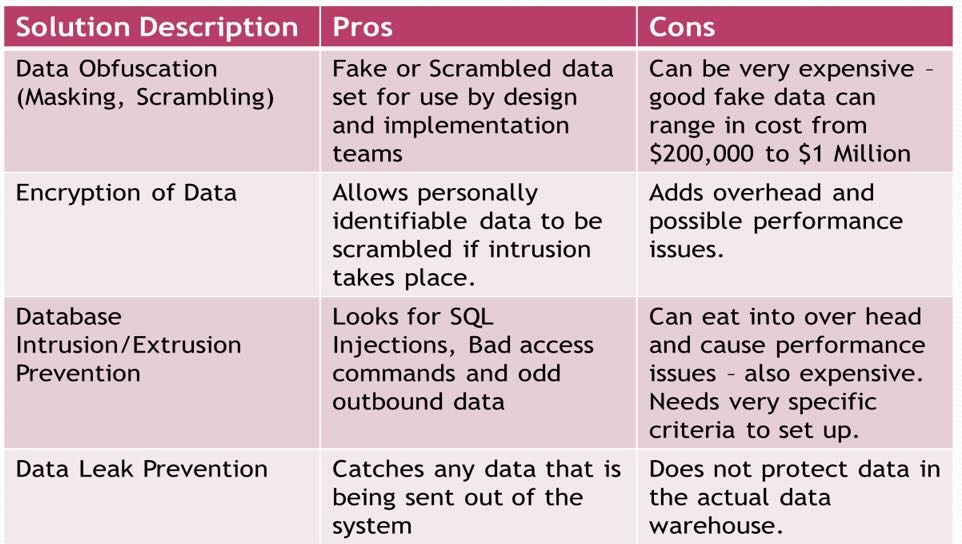
\includegraphics[scale=0.25]{security-solution-1.png}
	\end{center}
	\subsection{Using Built-in Solutions:}
	\begin{center}
		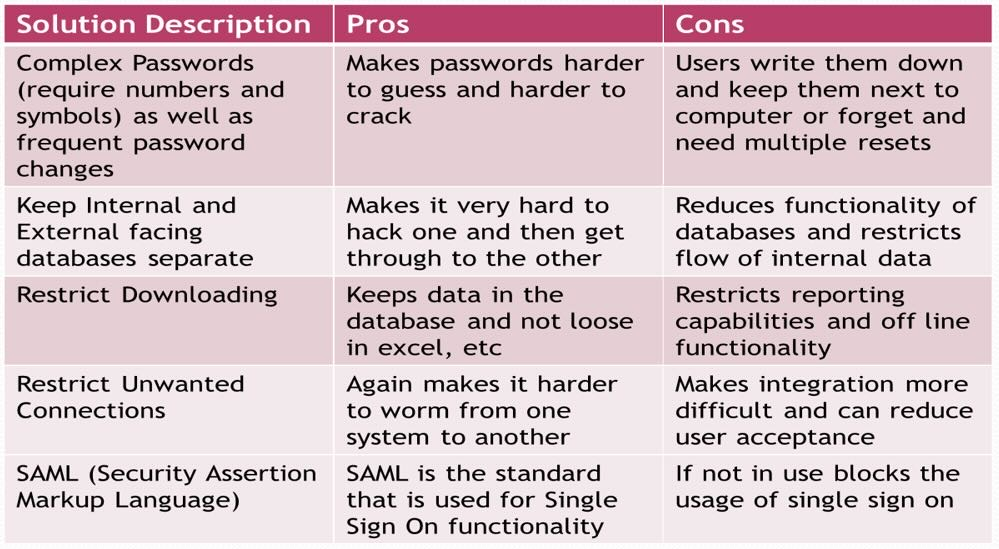
\includegraphics[scale=0.25]{security-solution-2.png}
	\end{center}
	\subsection{Privacy Facets:}
	\begin{itemize}
		\item Anonymity: Concealing identity of an entity
		\item Pseudonymity: Concealing true idenity of an entity
		\item Fair Use: Data collection relevant to the context
		\item Access: Limited access to dhe data
		\item Control Aggregation: Restricted distribution and appropiate sentitization
		\item Control Lifecycle: Data operationalization management
	\end{itemize}
	\subsection{Privacy Issues:}
	Using cloud services
	\begin{itemize}
		\item Entities outside of the organization now store and compute the data
		\item Attackers target the link between the cloud and client
		\item Cloud provider can now be phished
		\item Hard to audit data security
		\item Who is responsible for the when it leaks?
		\item Cloud can sub-contract to a third party organization
	\end{itemize}

	\section{Machine Learning Applications}
	\subsection{Watershed Moment:}
	In November 2016, Google integrated a multilingual nueral machine translation into Google translate. One of the first large-scale successful uses of deep nueral networks. This caused international interest for to adopt ML.
	\subsection{Evolution of Machine Learning:}
	ML is used everywhere within life. While most people think ML is just an algorithm, that is only one part of it. Complete ML systems also include business requirements, UI/UX, data pipelines and infrastructure which supports them.
	\subsection{When to use Machine Learning?:}
	ML is a powerful tool, but not always the best solution. It must first be considered whether it is truly necessary or cost-effective before starting a ML project.
	\subsection{Learn:}
	The most important step in ML. ML systems require large amounts of data to learn. In supervised learning, they learn from input-output pairs. This can then be used to predict output based on novel input.
	\subsection{Existing Data:}
	ML models can be deployed without prior training and use live data. This is known as continual learning. Deploying under trained models risks poor performance and bad UX.
	\subsection{Unseen Data:}
	The patterns a model learns on requires the assumption that the unseen data follow similar trends.
	\subsection{Where ML Works Best?:}
	The models work best when it's repetitive. This is becausethe patterns to be found are repeated multiple times. Also when the cost of wrong prediction is cheap. Good uses include Movies, music and clothes recommendations. Rather then Health data, Tesla's FSD.
	\subsection{ML vs Traditional Software:}
	\begin{center}
		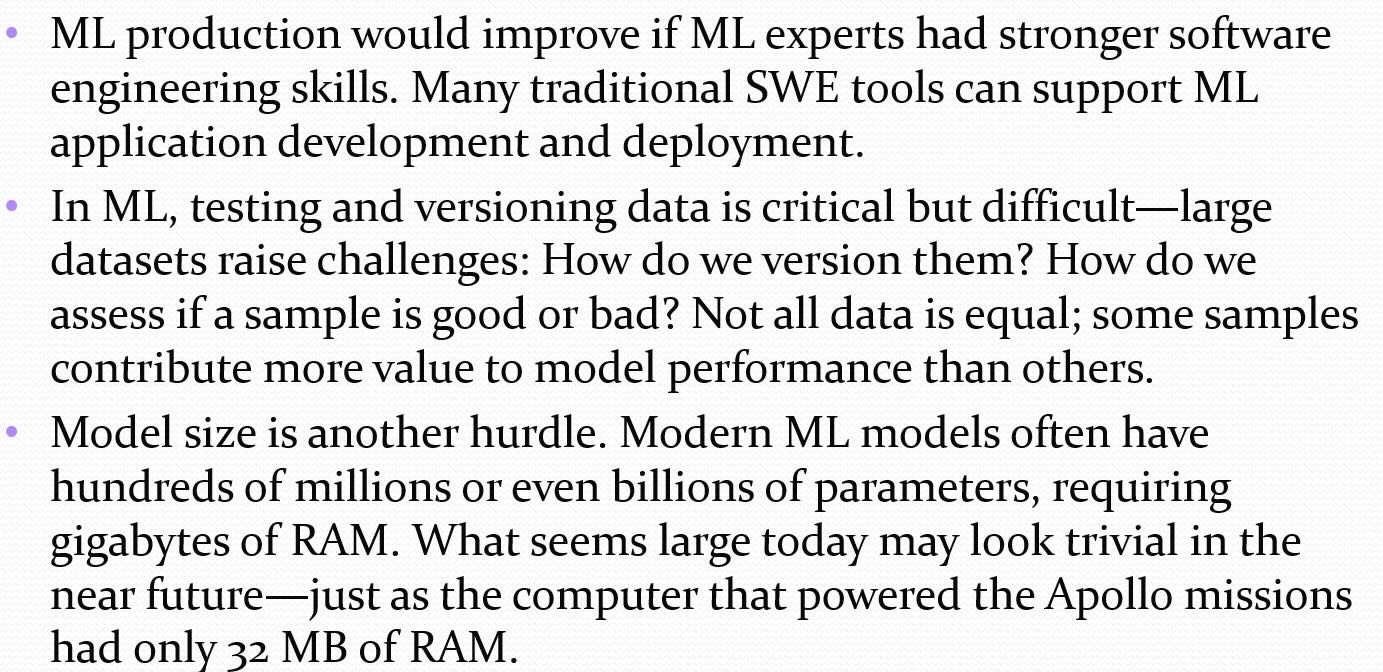
\includegraphics[scale=0.25]{ml-vs-trad-software.png}
	\end{center}
\end{document}
